%----------------------------------------------------------------------------------
% Arquivo template *.tex para TCC da Especialização em Ciência de Dados e Big Data
%----------------------------------------------------------------------------------

% Classe do documento.
\documentclass[12pt,a4paper]{article}

%-----------------------------------------------------------------------

\usepackage[brazil]{babel}
\usepackage[utf8]{inputenc}
\usepackage[a4paper,top=2.54cm,bottom=2.0cm,left=2.0cm,right=2.54cm]{geometry} % margens
\usepackage[pdftex,plainpages=false,pdfpagelabels,colorlinks=true,citecolor=blue,linkcolor=black,urlcolor=black,filecolor=red]{hyperref} 
\usepackage{multirow}
\usepackage{multicol}
\usepackage{natbib}
\usepackage{fancyhdr}
\usepackage{graphicx}
\usepackage{float}
\usepackage{pgfplots}
\usepackage{pgfplotstable}
\usepackage{tikz}
\usepackage{forest}
\usepackage{amsmath}
\pgfplotsset{compat=1.16}
\usetikzlibrary{fit,positioning,trees}

%-------------------------------------------------------------------------------%
% Corpo do texto
\begin{document}

%-------------------------------------------------------------------------------%
% Capa
% ---------------------------------------------------------------------------- %


\thispagestyle{empty}
\newcommand{\autor}{Carlos Magno Santos Ribeiro de Brito}
\newcommand{\orientador}{Eduardo Furtado de Simas Filho}
\newcommand{\titulo}{Análise de sentimentos em avaliações de clientes do \textit{e-commerce} nacional e comparação de métodos tradicionais de \textit{machine learning} com Redes Neurais \textit{Long Short Term Memory} (LSTM)}
\begin{center}

    \vspace*{2.3cm}
    \textbf{\Large{\titulo}}\\
    
    \vspace*{1.2cm}
    \Large{\autor}
    
    \vskip 2cm
    \textsc{
        Trabalho de Conclussão de Curso \\[-0.25cm]
        Apresentado ao\\[-0.25cm]
        Instituto de Matemática e Estatística\\[-0.25cm]
        da\\[-0.25cm]
        Universidade Federal da Bahia\\[-0.25cm]
        para\\[-0.25cm]
        obtenção do título\\[-0.25cm]
        de\\[-0.25cm]
        Especialista em Ciência de Dados \\ e Big Data}
    
    \vskip 1.5cm
    Orientador: Prof. Dr. \orientador \\
    
    \vskip 1cm
    \normalsize{Durante o desenvolvimento desta tese e curso o autor do presente trabalho foi contemplado com uma bolsa para realização da especialização}
    
    \vskip 2.5cm
    \normalsize{Salvador, \today}
\end{center}

% ---------------------------------------------------------------------------- %
% Página de rosto (só para a versão final)
% ---------------------------------------------------------------------------- %

%\newpage
%\thispagestyle{empty}
%\begin{center}
%\vspace*{2.3 cm}
%\textbf{\Large{Título}}\\
%\vspace*{2 cm}
%\end{center}
%
%\vskip 2cm
%
%\begin{flushright}
%
%Esta versão definitiva do trabalho de conclusão de curso\\
%contém as correções e alterações sugeridas pela\\
%Comissão Julgadora durante a defesa realizada\\
%por \textit{nome do alunos} em 02/12/2022.
%
%\vskip 2cm
%
%\end{flushright}
%\vskip 4.2cm
%
%\begin{quote}
%\noindent Comissão Julgadora:
%
%\begin{itemize}
%\item Profa. Dr. Fulano (orientadora) - IME-UFBA
%\item Prof. Dr. 
%\item Prof. Dr. 
%\end{itemize}
%
%\end{quote}
\pagebreak

% ---------------------------------------------------------------------------- %
\pagestyle{fancyplain}
\fancyhf{}
\lhead{\fancyplain{}{Especialização em Ciência de Dados e Big Data - ECD}}
\rhead{\fancyplain{}{\href{http://www.ecd.ufba.br}{\textit{www.ecd.ufba.br}}}}
\rfoot{\thepage}
\setcounter{page}{1}

\hspace{1.5em}

\begin{center}
    {\large \textbf{\titulo}}
\end{center}

\begin{flushleft}
    \textbf{\autor}\footnote{Universidade Federal da Bahia, \textit{carlos.ribeiro.brito@hotmail.com}} \\
    \textbf{\orientador}\footnote{Departamento de Engenharia Elétrica e de Computação, \textit{eduardo.simas@ufba.br}}\\
\end{flushleft}

\hspace{0.5em}
\hrule

\begin{center}
    {\large \textbf{Resumo}}
\end{center}
Com o advento do coronavirus no mundo, o e-commerce e todo o comércio \textit{on-line} no Brasil entre 2020 e 2021 se expandiu e se tornou ainda mais competitivo. Nesse contexto, identificar as necessidades dos consumidores e prever tendencias de expansão de vendas é uma necessidade dos empreendedores no mercado atual para se tornar mais competitivo. Tendo como base isso, o presente trabalho objetivou analisar e comparar dados de diferentes E-commerces no Brasil com diferentes tipos de modelos conhecidos da ciência de dados, na inteção de que os negócios possam ter bons \textit{tradeoffs} de seus modelos em aplicações e direcionar suas vendas de acordo com as preferências dos consumidores em diferentes nichos de mercados. Somando-se a isso, buscou-se indiretamente, desenvolver competências necessárias a prática profissional do cientista de dados, o qual projeta modelos e mecanismos de aprendizado orientados para os negócios e utiliza técnicas matemáticas para encontrar soluções de problemas de negócio ou científico.

\begin{flushleft}
    {\large \textbf{Palavras chaves:}} E-commerce; Machine Learning; Redes Neurais Artificiais.
\end{flushleft}

\hrule
\hspace{0.5em}

% ---------------------------------------------------------------------------- %
\section{Introdução}
\label{sec:intro}

O \textit{E-commerce}, ou comércio eletrônico, pode ser definido como uma modalidade de negócio onde todo o processo de compra é feito exclusivamente online, isto é, em aplicativos móveis e computadores é realizado desde a escolha do produto ao pagamento. O comércio eletrônico  como conhecemos hoje iniciou no final da década de 1960, mas desde 1993, novas tecnologias permitem as empresas realizar  funções de negócios eletrônicos (e-business) com maior eficiência, rapidez e  menores custos. Dados mais recentes da Associação Brasileira de Comércio  Eletrônico (ABComm) estimam que, em 2020, 20,2 milhões de consumidores realizaram uma compra on-line pela primeira vez e 150 mil lojas começaram a  vender por meio das plataformas digitais. Foram mais de 342 milhões de  negociações feitas pela internet, com um valor médio de R$\$ 310$ e um volume financeiro estimado de R$\$ 106$ bilhões \citep{Abcomm2020}.

Até pouco tempo atrás as lojas virtuais eram utilizadas como plataforma  de ampliação de vendas de lojas físicas já renomadas, à exemplo de Casas  Bahia, Magazine Luiza, Lojas Americanas e etc., mas com a crescente do e-commerce no Brasil nos anos de 2020 e 2021, proveniente da crise do  coronavírus, observa-se que as empresas estão apostando em lojas virtuais para  a exposição e vendas dos seus produtos, dispensando, muitas vezes, o comercio  em lojas físicas.

Por se tratar de um mercado de acesso nacional, com maior eficiência, rapidez e menores custos, a ocorrência das vendas on-line é elevada. Logo, para uma  empresa se manter competitiva e sólida neste mercado é preciso planejamento,  inovação e, principalmente, entender sobre as necessidades dos clientes e como  fidelizá-los. De acordo com \cite{Efagundes2021} um empreendimento de sucesso é aquele que  consegue utilizar a tecnologia existente, adequada aos consumidores do seu  nicho de mercado. Por isso mesmo, é  fundamental conhecer o comportamento dos consumidores e as tendencias do negócio.

No lado de quem consome, pode-se citar como vantagens do e-commerce: comodidade para os  clientes, acesso a opinião de outros usuários/compradores, funcionamento em tempo integral, diversidade de produtos, variedade de opções de pagamentos,  privacidade ao usuário/comprador, cupons de desconto e etc., e são justamente  estas vantagens e diversidades de informações de dados na compra e venda de  produtos que permitem identificar os nichos de mercados de cada seguimento.

Ainda no que concerne o consumidor, após a efetivação da compra, é solicitado uma avaliação do item. Ao se avaliar com pouca precisão, sem muito critério, ou sem muito zelo, algumas situações podem ser encotradas. A primeira delas é a condição não pouco incomum de uma nota desalinhada com o comentário avaliativo, por exemplo: é possível encontrar notas objetivas elevadas (escala 1 a 5, uma nota 5), porém com comentários que demonstram insatisfação com o produto. A segunda situação diz respeito às avaliações intermediárias, no que caracteriza o que é conhecido como \textit{j-shape rating}. Os usuários plenamente satisfeitos e/ou insatisfeitos tendem a avaliar o produto corretamente, todavia, o restante deles muitas vezes acabam avaliando sem muita convicção e de forma errônea.

Destarte, vista as condições de imprecisão ao se obter essas métricas em específico, com este trabalho objetivou analisar dados de diferentes \textit{e-commerces} no Brasil, mais especificamente as notas e comentários avaliativos dos produtos com intuito de obter uma classificação pertinente da satisfação do cliente e também um tradeoff entre assertividade e custo de processamento do modelo. Nesse processo foram concebidos modelos com cinco métodos tradicionais do aprendizado de máquina utilizados, sendo eles a Regressão logística, \textit{Naive Bayes}, \textit{XGBoost}, Florestas Aleatórias, \textit{LightGBM} e, para fins comparativos analisou-se também um modelo construído com rede neural artificial \textit{long short term memory} (LSTM).

% ---------------------------------------------------------------------------- %

% ---------------------------------------------------------------------------- %
\section{Materiais e métodos}
\label{sec:materials}

\subsection{Tipo de pesquisa}

Para realização deste trabalho, realizou-se uma pesquisa quantitativa descritiva, uma vez que buscou-se analisar dados de forma minuciosa a partir de Databases seccionados e coletados de diversas lojas virtuais no Brasil. Isto é, a pesquisa descritiva compreende a observação, ao registro, a análise, a classificação, a interpretação e a padronização de dados com a finalidade de explicar a correspondência entre as variáveis investigadas.

Em relação ao tratamento do problema, a pesquisa se caracterizou como quantitativa. Segundo \cite{malhotra2006pesquisa}, o objetivo da pesquisa quantitativa é quantificar os dados e aplicar ferramentas de análises estatísticas. O trabalho utilizou da tratativa, analise, correlação e apresentação de dados, além de aplicações de métodos estatísticos para criação de diferentes cenários, os quais têm como objetivo identificar possíveis tendência entre os dados utilizados e a satisfação do cliente na tomada de decisão em empresas que atuam nesse setor.

Quanto à coleta de dados, este trabalho foi classificado como uma pesquisa documental. A pesquisa documental recorre a fontes mais diversificadas e dispersas, sem tratamento analítico, tais como: tabelas estatísticas, jornais, revistas, relatórios, documentos oficiais, cartas, filmes, fotografias, pinturas, tapeçarias, relatórios de empresas, vídeos de programas de televisão, etc. \citep{fonseca2002}. A pesquisa documental é um tipo de pesquisa que é baseada dados e informações que não passaram por um processo analítico e/ou sintético. Os dados deste trabalho, de diferentes E-commerces no Brasil, foram disponibilizados pela Olist e estão disponíveis na plataforma \textit{Kaggle}, com o nome \textit{Brazilian E-Commerce Public Dataset} \citep{KaggleOlist}.

\subsection{Fonte e descrição dos dados}

Olist é uma startup brasileira que atua no segmento de E-commerce, sobretudo por meio de \textit{marketplace}. De um lado, a Olist concentra vendedores que desejam anunciar em \textit{marketplaces} como Mercado Livre, B2W, Via Varejo, Amazon e etc. Por outro, concentra os produtos de todos os vendedores em uma loja única que fica visível ao consumidor final. Atualmente o negócio reúne mais de 800 colaboradores e mais de 9 mil lojistas, além de 2 milhões de consumidores únicos \citep{Olist}.

A base de dados escolhida é um database público que consiste em um conjunto de dados que descrevem a rotina de compra de um E-commerce. É possível visualizar diversas características de um produto, como o nome, preço, descrição, nota atribuída, comentários, local de compra, etc. Mais especificamente, para este trabalho, analisou-se os comentários avaliativos (\textit{review\_comment\_message}) e as notas dadas pelos clientes (\textit{review\_score}). O tamanho total do dataset é de aproximadamente 126 \textit{megabytes} e da tabela que \textit{olist\_order\_review} com  14,45 \textit{megabytes} e aproximadamente 100 mil linhas.

\subsection{Ferramentas}

Abaixo na \autoref{fig:process}, tem-se o fluxograma do processo de realização deste trabalho. inicialmente a coleta de dados foi iniciada pelo Olist e assim disponibilizada a público. Em seguida, a análise e a sua validação é feita em trabalho, para verificar se os dados faziam sentido e se tinham a consistência informada. A análise dos resultados se deu após as análises do algoritmo produzido em \textit{python} juntamente com gráficos. As conclusões são feitas no presente trabalho, levando em conta o que foi proposto em ser analisado.

\begin{figure}[H]
    \centering
    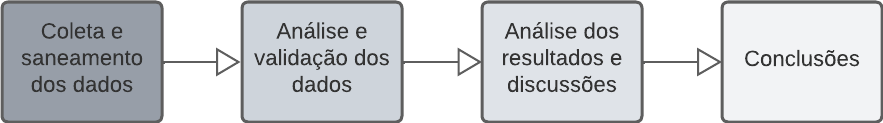
\includegraphics[width=\linewidth, scale=0.6]{./figs/process_diagram.png}
    \caption{Fluxograma do trabalho}
    \label{fig:process}
\end{figure}

O esquema dos \textit{databases} disponibilizados pelo Olist é representado na \autoref{fig:dataset_schema}. Nele, utilizou-se apenas a tabela \textit{olist\_order\_review}, com os campos disponíveis na \autoref{tab:review}. Além dele, o exemplo de como o cliente avalia um produto também é apresentado na \autoref{fig:review_ex}.

\begin{table}[H]
    \small
    \begin{tabular}{ccccc}
        \hline
        { }     & { review\_id}   & { order\_id}   & { review\_comment\_title} & { review\_comment\_message} \\ \hline
        { type} & { hash}         & { hash}        & { string|null}            & { string|null}              \\
        { ex}   & { da79b0a377eb} & { df73dbeba33} & { bom, mas}               & { atende às expectativas}   \\ \hline
    \end{tabular} \ldots
    \newline
    \vspace*{0.5 cm}
    \newline
    \begin{tabular}{cccc}
        \hline
        { }     & { review\_score} & { review\_creation\_date} & { review\_answer\_timestamp} \\ \hline
        { type} & { number}        & { datestring}             & { datestring}                \\
        { ex}   & { 3}             & { 2018-01-18 00:00:00}    & { 2018-01-18 21:00:00}       \\ \hline
    \end{tabular}
    \caption{Esquema da tabela \textit{olist\_order\_review}}
    \label{tab:review}
\end{table}

\begin{figure}[H]
    \centering
    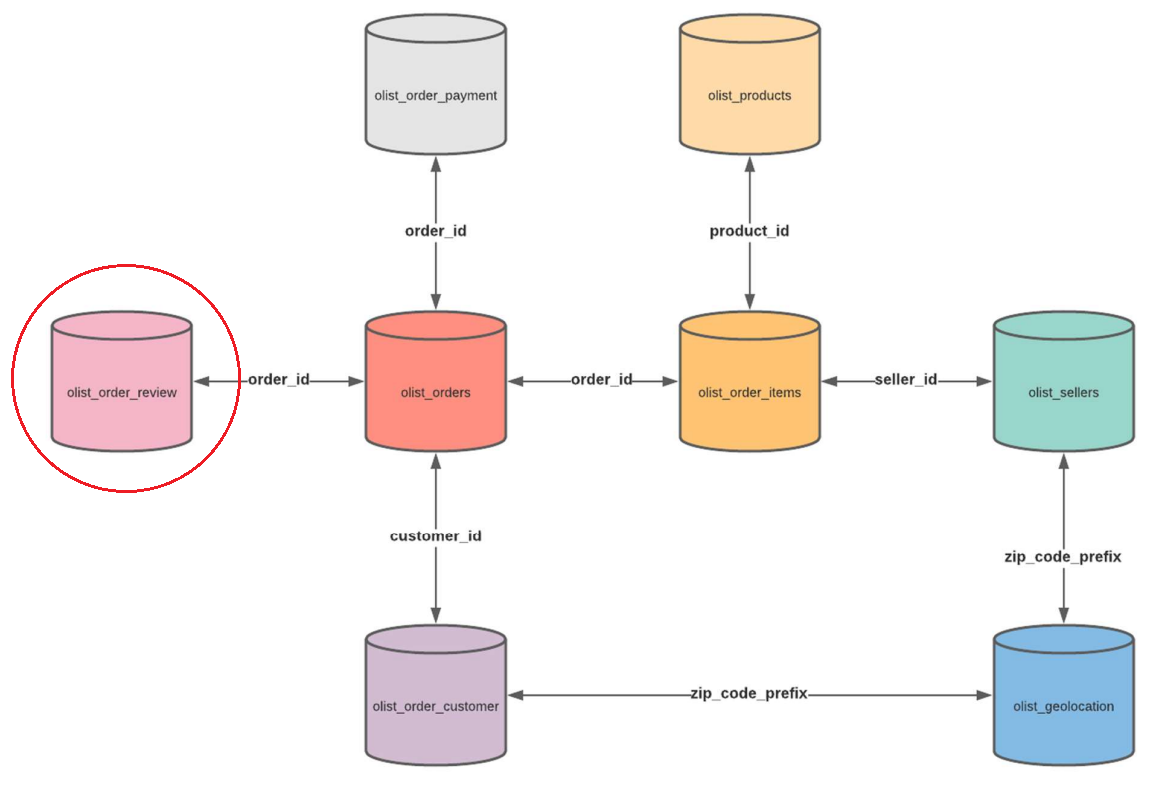
\includegraphics[scale=0.52]{./figs/database_schema.png}
    \caption{Esquemas do dataset publicado pelo Olist, adaptado pelo autor (2022)}
    \label{fig:dataset_schema}
\end{figure}

\begin{figure}[H]
    \centering
    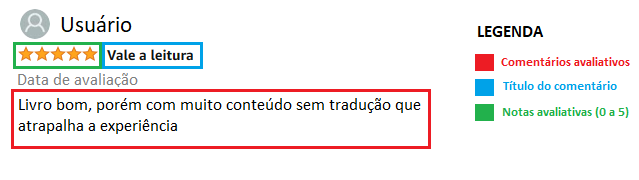
\includegraphics{./figs/review_ex.png}
    \caption{Forma de avaliação de um consumidor}
    \label{fig:review_ex}
\end{figure}


Na primeira fase, utilizando a linguagem de programação Python, os databases em formato CSV foram extraídos e exportados para leitura e armazenamento em diferentes variáveis no intuito de limpar e adequar os dados para análises. Nesta etapa, itens duplicados, com valores nulos e valores discrepantes foram removidos. Além disso, separou-se dois \textit{datasets} contendo informações dos comentários dos clientes (\textit{review\_comment\_message}) e da sua nota de avaliação (\textit{review\_score}). Para o \textit{data\_bin} tem-se comentários associados categoricamente com valores binários (0 e 1) a partir das notas, com o valor atribuído de 0 para o intervalo (0,2] e de 1 para o intervalo de (2, 5]. No \textit{data\_cat} tem-se apenas os comentários e os reviews numéricos de 1 a 5. Ambas as bases são removidos os valores nulos. Tem-se a \autoref{tab:bin} e \autoref{tab:gen} exemplificando os casos citados.


\begin{table}[H]
    \centering
    \begin{tabular}{cccc}
                & index  & text               & label   \\\hline\hline
        type    & bigint & string             & boolean \\\hline
        exemplo & 1      & produto muito ruim & 0
    \end{tabular}
    \caption{Esquema de geração do \textit{data\_bin}}
    \label{tab:bin}
\end{table}

\begin{table}[H]
    \centering
    \begin{tabular}{cccc}
                & index  & text              & label  \\\hline\hline
        type    & bigint & string            & number \\\hline
        exemplo & 2      & produto muito bom & 4
    \end{tabular}
    \caption{Esquema de geração do \textit{data\_gen}}
    \label{tab:gen}
\end{table}


\subsubsection{Máquina para processamento}

Todos os métodos foram executados em fila, sequencialmente entre eles, onde cada um deles foi executado em ordem, um de cada vez e de maneira procedural.

A máquina utilizada para todos eles foi o laptop Dell G3 com processador Intel Core i7 de 10ª geração, 16GB de RAM, 512GB de SSD e placa de vídeo NVIDIA RTX 2060 com 6GB de memória dedicada, incluindo o sistema operacional Windows 11 com WSL 2 instalado e Ubuntu 20.04 como ambiente de execução para as ferramentas de teste de software usadas.


\subsection{Métodos}

A partir das limpeza dos dados, para análise de ambos datasets gerados, lançou-se mão de métodos clássicos do \textit{Machine learning} sendo eles: Regressão logística, Naive Bayes, Florestas Aleatórias e \textit{XGBoost}. Além deles, para comparação, utilizou-se uma rede neural artificial LSTM. Esses métodos serão aqui melhor detalhados.

% Regressão logística

\subsubsection{Regress�o Log�stica}

A regress�o log�stica � um modelo estat�stico robusto e eficiente, que permite a previs�o da probabilidade de um evento bin�rio de forma precisa e confi�vel \citep{hosmer2013applied}. Este tipo de evento � aquele que pode ocorrer ou n�o, ou que pode ser classificado em duas categorias distintas. Por exemplo, em uma an�lise de cr�dito, o cliente pode ser aprovado ou n�o. Na medicina, o evento pode ser a cura ou n�o de uma doen�a.

Ela apresenta um modelo linear generalizado que utiliza a fun��o log�stica para modelar a rela��o entre as vari�veis independentes e a vari�vel dependente \citep{kleinbaum2010logistic}. A fun��o log�stica � uma fun��o sigmoide que transforma uma vari�vel linear em uma probabilidade. A equa��o da fun��o log�stica � dada por:

\begin{equation}
    p = \frac{1}{1 + e^{-x}}
\end{equation}

Sendo $p$ a probabilidade do evento ocorrer, $x$ uma vari�vel linear que representa a combina��o linear das vari�veis independentes, e $e$ a constante de Euler.

A regress�o log�stica utiliza a t�cnica de m�xima verossimilhan�a para estimar os par�metros do modelo a partir dos dados observados. A fun��o de verossimilhan�a � maximizada para encontrar os valores dos coeficientes que melhor se ajustam aos dados. O modelo � ajustado para minimizar a diferen�a entre as probabilidades previstas pelo modelo e as probabilidades observadas nos dados \citep{mccullagh1989generalized}.

A regress�o log�stica tem sido amplamente utilizada em diversas �reas, como na an�lise de dados de sobreviv�ncia, na an�lise de dados de sa�de, na an�lise de dados financeiros, etc. Por exemplo, � utilizada na an�lise de dados de sobreviv�ncia para modelar a probabilidade de um paciente sobreviver a uma doen�a com base em fatores como idade, sexo, n�vel de educa��o, etc. Na an�lise de dados financeiros, � utilizada para modelar a probabilidade de um cliente pagar ou n�o uma d�vida com base em fatores como hist�rico de cr�dito, renda, etc.


\input{./tikz/logistic.tikz.tex}

% Classificação Naive Bayes

\subsubsection{Naive Bayes}

A classifica��o Naive Bayes � um algoritmo de aprendizado de m�quina supervisionado que utiliza o teorema de Bayes para classificar inst�ncias em classes discretas. A principal vantagem do algoritmo Naive Bayes � a sua simplicidade e efici�ncia computacional, o que o torna uma escolha popular para problemas de classifica��o em grande escala \citep{mitchell1997machine}.

O algoritmo Naive Bayes � baseado no teorema de Bayes, que fornece uma maneira de calcular a probabilidade condicional de uma hip�tese, dado um conjunto de evid�ncias. Na classifica��o, a hip�tese corresponde � classe da inst�ncia e as evid�ncias correspondem �s caracter�sticas observadas da inst�ncia. O algoritmo calcula a probabilidade condicional de cada classe, dado as caracter�sticas observadas da inst�ncia, e atribui a inst�ncia � classe com a maior probabilidade condicional.

Segundo \cite{domingos1997optimality}, a principal suposi��o por tr�s do algoritmo Naive Bayes � a independ�ncia condicional das caracter�sticas, ou seja, cada caracter�stica contribui independentemente para a probabilidade condicional de cada classe. Embora essa suposi��o seja muitas vezes violada na pr�tica, o algoritmo Naive Bayes ainda funciona bem em muitos casos e pode ser especialmente �til quando h� muitas caracter�sticas.

O algoritmo Naive Bayes tem sido aplicado em muitas �reas, incluindo reconhecimento de fala, processamento de texto e detec��o de spam de e-mail. � particularmente �til em aplica��es onde h� muitas caracter�sticas e as inst�ncias s�o discretas ou categ�ricas. Um estudo emp�rico sobre o desempenho do algoritmo Naive Bayes em diferentes conjuntos de dados pode ser encontrado em \citep{rish2001empirical}.

Embora o algoritmo Naive Bayes seja uma t�cnica de classifica��o simples e eficiente, ele tamb�m tem algumas limita��es. Por exemplo, a suposi��o de independ�ncia condicional das caracter�sticas pode ser inadequada em algumas situa��es, e a performance do algoritmo pode ser afetada por dados ausentes ou dados ruidosos \citep{mitchell1997machine}.

As equa��es abaixo representam a base matem�tica do algoritmo de classifica��o Naive Bayes:

Dada uma inst�ncia $X = {x_1, x_2, \dots, x_n}$ com caracter�sticas observadas, o objetivo do algoritmo � determinar a probabilidade condicional $P(C_k|X)$ da inst�ncia pertencer a cada classe $C_k$.

O teorema de Bayes fornece uma maneira de calcular a probabilidade condicional $P(C_k|X)$ em termos das probabilidades a priori $P(C_k)$ e das probabilidades condicionais $P(X|C_k)$, como segue:

\begin{equation}
    P(C_k|X)=\frac{P(X|C_k)P(C_k)}{P(X)}
\end{equation}

Aqui, $P(C_k)$ � a probabilidade a priori da classe $C_k$ e $P(X|C_k)$ � a probabilidade condicional de observar a inst�ncia $X$ dada a classe $C_k$.

O classificador Naive Bayes assume a independ�ncia condicional das caracter�sticas dadas a classe, isto �, $P(x_i|C_k, x_1, \dots, x_{i-1}, x_{i+1}, \dots, x_n) = P(x_i|C_k)$. Isso permite simplificar a probabilidade condicional $P(X|C_k)$ como:

\begin{equation}
    P(X|C_k)=P(x_1, \dots, x_{i-1}, x_{i+1}, \dots, x_n|C_k)=\prod_{i=1}^{n}P(x_i|C_k)
\end{equation}

Substituindo essa express�o na equa��o anterior, tem-se:

\begin{equation}
    P(C_k|X)=\frac{\prod_{i=1}^{n}P(x_i|C_k)P(C_k)}{P(X)}
\end{equation}

Como a probabilidade $P(X)$ � constante para todas as classes, � poss�vel comparar apenas as probabilidades $P(C_k)\prod_{i=1}^n P(x_i|C_k)$ para determinar a classe mais prov�vel para a inst�ncia $X$.

O desenho ilustra as vari�veis aleat�rias $x_1, x_2, x_3, x_4$ e a classe $C_k$. As setas que partem das probabilidades condicionais e a priori indicam as f�rmulas para o c�lculo das probabilidades conjuntas $P(x_1, x_2, x_3, x_4, C_k)$ e, consequentemente, para a classifica��o de uma inst�ncia.

\input{./tikz/bayes.tikz.tex}

% Florestas aleatórias

\subsubsection{Florestas aleat�rias}

De acordo com \cite{breiman2001random}, as florestas aleat�rias s�o uma t�cnica de aprendizado de m�quina que combina v�rias �rvores de decis�o para construir um modelo de classifica��o ou regress�o. Cada �rvore de decis�o � constru�da a partir de um subconjunto aleat�rio dos dados de treinamento e um subconjunto aleat�rio dos recursos (tamb�m conhecidos como caracter�sticas ou atributos). Esses subconjuntos s�o criados para garantir que cada �rvore de decis�o seja diferente e que a floresta aleat�ria possa capturar v�rias rela��es entre os dados e recursos.

A constru��o de uma �rvore de decis�o � feita por meio de uma s�rie de etapas. Inicialmente, a �rvore come�a com um �nico n� que representa todo o conjunto de dados de treinamento. Em seguida, a �rvore � dividida em n�s menores usando uma fun��o de divis�o que escolhe um recurso e um ponto de divis�o que minimiza a impureza dos dados. A impureza � uma medida da desorganiza��o dos dados, que pode ser medida por diferentes crit�rios, como a entropia ou o �ndice Gini. O processo de divis�o � repetido recursivamente at� que os n�s finais sejam puros ou um crit�rio de parada seja atingido, como uma profundidade m�xima da �rvore \citep{cutler2001random}.

Durante a fase de teste, a floresta aleat�ria retorna a classe mais comum ou a m�dia das sa�das das �rvores individuais, dependendo se o problema � de classifica��o ou regress�o, respectivamente.

As florestas aleat�rias apresentam v�rias vantagens em rela��o a outras t�cnicas de aprendizado de m�quina. Em primeiro lugar, elas t�m um bom desempenho em dados de alta dimens�o, onde o n�mero de recursos � grande em rela��o ao n�mero de amostras. Em segundo lugar, elas s�o relativamente insens�veis a outliers e dados ausentes. Em terceiro lugar, elas s�o facilmente paraleliz�veis, permitindo que grandes conjuntos de dados sejam processados em paralelo em clusters de computadores \citep{cutler2001random}.

Em termos de aplica��o, elas s�o amplamente utilizadas em uma variedade de problemas, como reconhecimento de padr�es em imagens e sinais, detec��o de fraudes em transa��es financeiras, an�lise de sentimentos em redes sociais, previs�o de pre�os de a��es e an�lise de dados gen�micos \citep{breiman2001random}.

As equa��es relacionadas �s florestas aleat�rias s�o principalmente as usadas na constru��o de cada �rvore de decis�o. Por exemplo, as equa��es para o c�lculo da impureza dos dados, que � um dos principais crit�rios de divis�o de n�s em uma �rvore de decis�o s�o dadas:

\begin{itemize}
    \item O �ndice Gini:
          \begin{equation}
              G_i = \sum_{k=1}^{K} p_{i,k} (1-p_{i,k}),
          \end{equation}

          onde $K$ � o n�mero de classes, $p_{i,k}$ � a propor��o de observa��es da classe $k$ no n� $i$.
    \item A entropia:
          \begin{equation}
              H_i = -\sum_{k=1}^{K} p_{i,k} \log(p_{i,k}),
          \end{equation}

          onde $K$ � o n�mero de classes, $p_{i,k}$ � a propor��o de observa��es da classe $k$ no n� $i$.

    \item O crit�rio de divis�o de Gini � dado por:
          \begin{equation}
              G_{d} = \sum_{i=1}^{q}\frac{n_i}{n}G_i,
          \end{equation}

          onde $q$ � o n�mero de n�s filhos resultantes da divis�o, $n_i$ � o n�mero de observa��es no n� $i$ e $n$ � o n�mero total de observa��es.

    \item O crit�rio de divis�o de entropia � dado por:
          \begin{equation}
              H_{d} = -\sum_{i=1}^{q}\frac{n_i}{n}H_i,
          \end{equation}

          onde $q$ � o n�mero de n�s filhos resultantes da divis�o, $n_i$ � o n�mero de observa��es no n� $i$ e $n$ � o n�mero total de observa��es.

\end{itemize}

Essas equa��es s�o usadas para calcular a impureza dos dados em cada n� da �rvore de decis�o e, assim, decidir qual recurso e ponto de divis�o usar para dividir o n� em dois filhos. O processo de divis�o � repetido recursivamente para construir a �rvore de decis�o completa. Em seguida, v�rias �rvores de decis�o s�o combinadas para formar a floresta aleat�ria.

\input{tikz/forest.tikz.tex}










% XGBoost

\subsubsection{XGBoost}

O XGBoost (\textit{Extreme Gradient Boosting}) � um m�todo de aprendizado de m�quina baseado em �rvores de decis�o, assim como as florestas aleat�rias, mas com algumas diferen�as importantes. Enquanto as florestas aleat�rias usam um conjunto de �rvores de decis�o independentes para fazer uma previs�o, o XGBoost usa um conjunto de �rvores de decis�o sequenciais que s�o criadas iterativamente. Cada nova �rvore � ajustada aos res�duos do modelo anterior, tentando corrigir os erros cometidos pelo modelo atual.

O algoritmo XGBoost foi desenvolvido por Tianqi Chen e Carlos Guestrin em 2016 \citep{Chen:2016} e � baseado na biblioteca de c�digo aberto de mesmo nome. O XGBoost se tornou um dos algoritmos de aprendizado de m�quina mais populares em competi��es de ci�ncia de dados e � amplamente utilizado na ind�stria.

O processo de constru��o do modelo XGBoost pode ser descrito por meio da seguinte equa��o:

\begin{equation}
    \hat{y_i} = \phi(\mathbf{x}_i) = \sum_{k=1}^{K}(\mathbf{x}_i)
\end{equation}

onde $\hat{y_i}$ � a previs�o para a i-�sima inst�ncia, $\phi$ � a fun��o de previs�o, $\mathbf{x}_i$ � o vetor de caracter�sticas para a i-�sima inst�ncia, $K$ � o n�mero total de �rvores no modelo e $f_k$ � a k-�sima �rvore de decis�o.

Para construir o modelo XGBoost, o algoritmo usa um processo iterativo de adi��o de �rvores, onde cada nova �rvore � ajustada aos res�duos do modelo anterior, tentando corrigir os erros cometidos pelo modelo atual. Esse processo � descrito pela seguinte equa��o:

\begin{equation}
    \mathbf{F}_k = \mathbf{F}_{k-1} + \gamma_k f_k
\end{equation}

onde $\mathbf{F}_k$ � a soma cumulativa das previs�es das �rvores anteriores at� a k-�sima �rvore, $\gamma_k$ � a taxa de aprendizado da k-�sima �rvore e $f_k$ � a k-�sima �rvore de decis�o.

O XGBoost tamb�m usa um conjunto de hiperpar�metros para ajustar o modelo e evitar overfitting. Alguns dos hiperpar�metros mais importantes incluem:

\begin{itemize}
    \item N�mero de �rvores: o n�mero total de �rvores a serem criadas;
    \item Profundidade m�xima: o n�mero m�ximo de camadas que cada �rvore pode ter;
    \item Taxa de aprendizado: a taxa na qual o modelo tenta corrigir os erros cometidos pelas �rvores anteriores;
    \item Subamostragem: a fra��o de amostras de treinamento a serem usadas para treinar cada �rvore;
    \item Colsample: a fra��o de recursos (caracter�sticas) a serem amostrados aleatoriamente para cada �rvore.
\end{itemize}

Chen e Guestrin descrevem o algoritmo XGBoost em detalhes em seu artigo "XGBoost: A Scalable Tree Boosting System" \citep{Chen:2016}, onde eles mostram que o XGBoost pode superar outros algoritmos de aprendizado de m�quina em uma variedade de conjuntos de dados e tarefas.

Uma das principais vantagens do XGBoost � sua efici�ncia computacional. O algoritmo usa v�rias t�cnicas para reduzir o tempo de treinamento e a complexidade do modelo, incluindo a amostragem de caracter�sticas, a paraleliza��o do processo de treinamento e o uso de uma estrutura de dados espec�fica chamada "gradiente e Hessiano".

O XGBoost � amplamente utilizado em competi��es de ci�ncia de dados e em projetos de aprendizado de m�quina na ind�stria. A biblioteca XGBoost � de c�digo aberto e est� dispon�vel para v�rias linguagens de programa��o, incluindo Python, R e Java.

As seguintes equa��es s�o usadas para calcular os valores dos gradientes e Hessiano para cada inst�ncia $i$:

\begin{equation}
    \begin{aligned}
         & g_i = \frac{\partial L (y_i, \hat{y_i})}{\partial \hat{y_i}},      \\
         & h_i = \frac{\partial^2 L (y_i, \hat{y_i})}{\partial \hat{y_{i}}^2}
    \end{aligned}
\end{equation}


onde $L$ � a fun��o de perda usada para avaliar a qualidade da previs�o. O XGBoost usa esses valores de gradiente e Hessiano para ajustar as �rvores do modelo, tentando minimizar a fun��o de perda.

% lightGBM

\subsubsection{lightGBM}

LightGBM é um algoritmo de aprendizado de máquina baseado em árvore, desenvolvido pela Microsoft, que utiliza um método de treinamento baseado em gradientes para melhorar a velocidade e a eficiência de modelos baseados em árvore. O algoritmo utiliza uma técnica de amostragem por folha, que pode levar a melhorias significativas no tempo de treinamento e na precisão do modelo.

Segundo \cite{ke2017lightgbm}, o LightGBM apresenta melhorias significativas em relação a outros algoritmos de aprendizado de máquina baseados em árvore, como o XGBoost, tanto em termos de tempo de treinamento quanto de desempenho preditivo. O LightGBM é particularmente eficaz em conjuntos de dados grandes e esparsos, e tem sido amplamente utilizado em aplicações de classificação e regressão.

Uma das principais vantagens do LightGBM é a sua eficiência computacional. Esta técnica de amostragem por folha, em que cada folha da árvore é treinada com um subconjunto aleatório dos dados de treinamento permite que o algoritmo treine árvores mais profundas e complexas sem aumentar significativamente o tempo de treinamento. Além disso, o LightGBM utiliza uma técnica de paralelização de histogramas, que divide os dados em intervalos discretos e constrói histogramas para cada recurso, permitindo que as operações de treinamento sejam executadas em paralelo.

O LightGBM também apresenta melhorias significativas no desempenho preditivo em relação a outros algoritmos de aprendizado de máquina baseados em árvore. \cite{ke2017lightgbm} mostraram que o LightGBM supera o XGBoost em várias métricas de desempenho, incluindo tempo de treinamento, tempo de previsão e precisão preditiva em vários conjuntos de dados. O LightGBM também é capaz de lidar com conjuntos de dados grandes e esparsos, que são comuns em muitas aplicações do mundo real.

Em relação às suas principais equações definidoras, tem-se:

A) A função objetivo (\textit{loss function}) utilizada pelo LightGBM que é dada por:
\begin{equation}
    L(\theta) = \sum_{i=1}^n l(y_i, f(\mathbf{x_i};\theta)) + \sum_{k=1}^K \Omega(f_k)
\end{equation}

Onde $l$ é a função de perda, $y_i$ é o rótulo do exemplo de treinamento $i$, $f(\mathbf{x_i};\theta)$ é a predição do modelo para o exemplo $\mathbf{x_i}$, $\theta$ é o conjunto de parâmetros do modelo, $K$ é o número de árvores utilizadas pelo modelo, e $\Omega(f_k)$ é a função de regularização utilizada para controlar a complexidade do modelo.

B) O algoritmo utiliza o método de boosting para construir o modelo. Em cada iteração $t$, o LightGBM adiciona uma nova árvore $f_t$ ao modelo. A predição do modelo após $T$ iterações é dada por:

\begin{equation}
    f_T(\mathbf{x}) = \sum_{t=1}^T f_t(\mathbf{x})
\end{equation}

C) A técnica de gradientes para atualizar os parâmetros do modelo em cada iteração. A atualização dos parâmetros é realizada utilizando o seguinte algoritmo:

\begin{enumerate}
    \item Computar os gradientes para cada exemplo de treinamento:
          \begin{equation}
              g_i = \frac{\partial l(y_i, f(\mathbf{x_i};\theta))}{\partial f(\mathbf{x_i};\theta)}
          \end{equation}
    \item Construir uma nova árvore $f_t$ que minimize a função objetivo:
          \begin{equation}
              f_t = \arg \min_{f} \sum_{i=1}^n g_i f(\mathbf{x_i};\theta_{t-1}) + \frac{1}{2} h f^2(\mathbf{x_i}) + \Omega(f)
          \end{equation}

          Onde $h$ é a taxa de aprendizagem (learning rate) utilizada para controlar a magnitude da atualização dos parâmetros.
\end{enumerate}

% Redes Neurais

\subsubsection{Redes Neurais}

\input{tikz/neuralNetwork.tikz.tex}

Redes Neurais Artificiais (RNAs) s�o modelos computacionais que se inspiram no funcionamento do c�rebro humano e t�m sido amplamente utilizadas para tarefas de classifica��o, previs�o e reconhecimento de padr�es em diferentes �reas do conhecimento. O conceito de RNA foi proposto por \cite{mcculloch1943logical}, mas foi apenas a partir da d�cada de 1980, com o desenvolvimento de t�cnicas de treinamento de redes profundas, que as RNAs se tornaram uma ferramenta poderosa para an�lise de dados \cite{lecun2015deep}.

Uma RNA � composta por camadas de neur�nios artificiais, cada um com uma fun��o de ativa��o que transforma a entrada recebida em uma sa�da. A primeira camada � a camada de entrada, que recebe os dados a serem processados. A �ltima camada � a camada de sa�da, que produz a resposta final da RNA. Entre as camadas de entrada e sa�da, podem ser adicionadas v�rias camadas ocultas, que ajudam a extrair caracter�sticas dos dados de entrada.

O processo de treinamento de uma RNA consiste em ajustar os pesos sin�pticos entre os neur�nios para que a rede produza a sa�da correta para cada entrada. O algoritmo mais comum de treinamento � o Backpropagation, proposto por \cite{rumelhart1986parallel}. O Backpropagation utiliza o m�todo do gradiente descendente para minimizar a fun��o de custo da RNA em rela��o aos pesos sin�pticos.

Uma das principais vantagens das RNAs � a capacidade de lidar com dados complexos e n�o lineares. Al�m disso, as RNAs podem ser utilizadas em problemas de classifica��o, previs�o e reconhecimento de padr�es em diferentes �reas, como vis�o computacional, processamento de fala, processamento de texto e bioinform�tica.

No entanto, as RNAs possuem algumas desvantagens, como a dificuldade de interpreta��o dos resultados e o risco de overfitting, que ocorre quando a rede se ajusta demais aos dados de treinamento e n�o consegue generalizar para novos dados.

As redes neurais artificiais s�o compostas por uma s�rie de camadas de neur�nios, que realizam opera��es matem�ticas nas entradas recebidas para gerar sa�das. A formula��o matem�tica dessas opera��es pode variar de acordo com a arquitetura da rede, mas em geral envolvem uma combina��o linear das entradas, seguida de uma fun��o n�o linear de ativa��o.

Abaixo tem-se as equa��es matem�ticas para uma rede neural \textit{feedforward} de tr�s camadas, com $n^{(l)}$ neur�nios na camada $l$:

\begin{equation}
    \begin{aligned}
         & z_j^{(2)} = \sum\limits_{i=1}^{n^{(1)}} w_{ij}^{(1)} x_i + b_j^{(1)}       \\
         & h_j^{(2)} = f(z_j^{(2)})                                                   \\
         & z_k^{(3)} = \sum\limits_{j=1}^{n^{(2)}} w_{jk}^{(2)} h_j^{(2)} + b_k^{(2)} \\
         & y_k = f(z_k^{(3)})
    \end{aligned}
\end{equation}

Na equa��o acima, $x_i$ representa a entrada na posi��o $i$, $w_{ij}^{(1)}$ representa o peso associado � conex�o entre o neur�nio $i$ da camada de entrada e o neur�nio $j$ da camada oculta, $b_j^{(1)}$ � o vi�s associado ao neur�nio $j$ da camada oculta, $f$ � a fun��o de ativa��o, $h_j^{(2)}$ � a sa�da do neur�nio $j$ da camada oculta, $w_{jk}^{(2)}$ � o peso associado � conex�o entre o neur�nio $j$ da camada oculta e o neur�nio $k$ da camada de sa�da, $b_k^{(2)}$ � o vi�s associado ao neur�nio $k$ da camada de sa�da e $y_k$ � a sa�da final da rede neural.

� importante notar que a escolha da fun��o de ativa��o pode influenciar significativamente o comportamento da rede neural, permitindo, por exemplo, que ela aprenda a modelar fun��es n�o-lineares complexas. Algumas fun��es de ativa��o comuns incluem a fun��o sigmoide, a fun��o tangente hiperb�lica e a fun��o ReLU (Rectified Linear Unit).










% ---------------------------------------------------------------------------- %

\section{Resultados}
\label{sec:results}

Após a limpeza dos dados, iniciou-se o processo de análise dos mesmos. Com isso, algumas considerações poderam ser tomadas. Como dito \textit{a priori}, por ser tão abrangente, essa análise foi limitada ao sistema de avaliação feito pelos clientes após a confirmação de entrega do produto. Assim, o consumidor pode dar nota de 1 a 5 para o produto, sendo 1 o mais baixo e 5 o mais alto.


\begin{figure}[H]
    \centering
    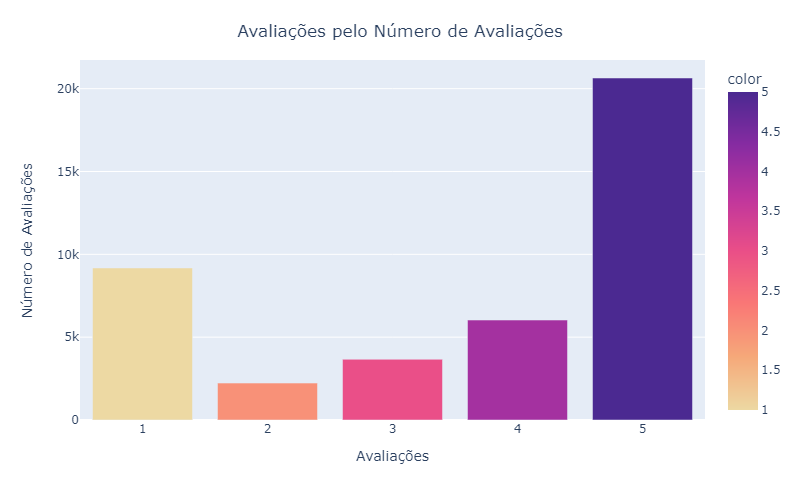
\includegraphics[trim={0cm 2cm 3cm 2cm},clip,scale=0.65]{./figs/eval.png}
    \caption{Distribuição das avaliações}
    \label{fig:evalDistribution}
\end{figure}

À primeira vista com o quantitativo de notas, é possível perceber que essa  distribuição é dada em forma de ``J" e é bastante típica em \textit{e-commerces}. Grande  quantidade de avaliações 5, 4 e 1, pequena quantidade de 2 e 3.

Este tipo de distribuição pode ocorrer por várias razões. Uma possível explicação é que os clientes que estão extremamente satisfeitos ou insatisfeitos com um produto são mais propensos a deixar uma avaliação do que aqueles que têm uma experiência neutra. Isso pode resultar em uma concentração maior de avaliações com classificações muito altas ou muito baixas.

Outra possível explicação é que os clientes que têm uma experiência neutra com um produto podem não se sentir motivados a deixar uma avaliação. Eles podem sentir que o produto foi bom, mas não excepcional, e, portanto, não vale a pena dedicar tempo para escrever uma avaliação. Isso pode levar a um menor número de avaliações com classificações médias.

A distribuição em forma de ``J" das avaliações pode ser importante para as empresas entenderem, pois pode fornecer informações sobre a satisfação do cliente e a qualidade do produto. Se um produto tiver uma alta concentração de avaliações muito positivas, pode ser um indicador de forte satisfação do cliente e um produto de alta qualidade. No entanto, também é importante considerar o número de avaliações e a média geral das classificações, já que um pequeno número de avaliações pode distorcer a distribuição.

Seguidamente, plotou-se a distribuição binária das avaliações conforme foi seccionado na etapa de tratamento dos dados. De forma coerente com a \autoref{fig:evalDistribution} e com a divisão adotada, a maior parte das avaliações são positivas.

\begin{figure}[H]
    \centering
    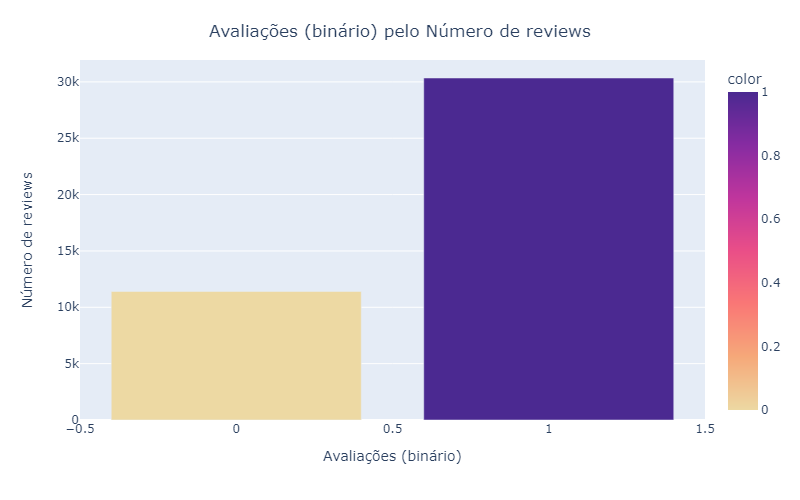
\includegraphics[trim={0cm 2cm 3cm 2cm},clip,scale=0.6]{./figs/bin_eval.png}
    \caption{Distribuição das avaliações binárias}
    \label{fig:binEvalDistribution}
\end{figure}

Uma nuvem de palavras então é gerada a partir de um conjunto de dados de texto referente aos comentários avaliativos dos clientes. As palavras são extraídas do texto e organizadas em uma nuvem, em que as palavras mais frequentes são maiores e as menos frequentes são menores. A nuvem de palavras pode ser usada para ajudar a identificar tópicos e padrões importantes em um conjunto de dados de texto e para comunicar visualmente essas informações.

\begin{figure}[H]
    \centering
    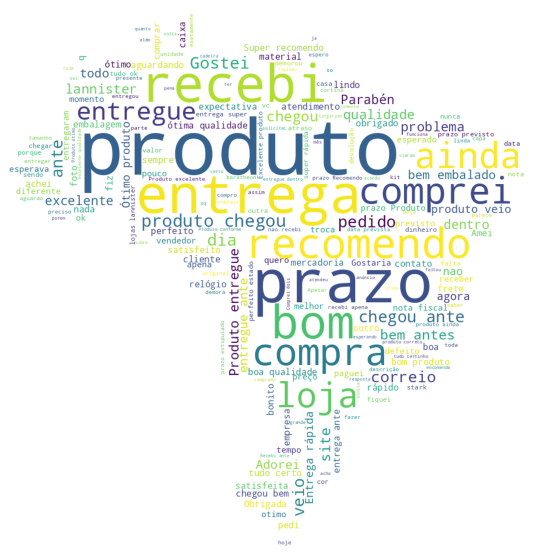
\includegraphics[scale=0.8]{./figs/word_cloud.png}
    \caption{Nuvem de palavras destacando os principais termos utilizados}
    \label{fig:wordCloud}
\end{figure}

Essa técnica visual pode ser usada em vários campos, incluindo análise de sentimentos, mineração de opiniões, análise de redes sociais, pesquisa de mercado e análise de \textit{feedback} de clientes como o caso em específico. Além disso, por ser uma forma visualmente atraente de resumir informações e destacar pontos importantes, é bastante útil para relatórios e análises.

Tendo feito a tokenização das palavras, isto é, um processo de transformação de todas as palabras de entrada em listas de numeros, filtrado pelas \textit{stopwords} e feito um processo de padronização textual, separou-se o \textit{dataset} entre treino e teste e prosseguiu para as demais análises com os algorítmos de aprendizado de máquina e redes neurais.

Dentre os algoritmos de aprendizado de máquina, encontrou-se as seguintes acurácias conforme a \autoref{tab:accur}.

\begin{table}[H]
    \centering
    \begin{tabular}{l|ccccc}
        \hline
        { modelo}      & { Reg. Logística} & { F. Aleatórias} & { XGBoost} & { Naive Bayes} & LightGBM \\ \hline\hline
        { treino (\%)} & { 73.9}           & { 99.6}          & { 93.5}    & { 74.0}        & 86.7     \\\hline
        { teste (\%)}  & { 73.3}           & { 78.2}          & { 82.1}    & { 74.0}        & 81.3
    \end{tabular}
    \caption{Comapração entre teste e treino nos modelos de aprendizado de máquina}
    \label{tab:accur}
\end{table}

Observa-se que nos modelos XGBoost e LightGBM os valores foram muito próximos e apresentaram os melhores resultados em teste.

A regressão logística tem um tempo de execução muito maior do que os outros modelos, o que pode ser um fator limitante em muitas aplicações. Por outro lado, o Naive Bayes tem um tempo de execução muito curto, mas também tem a menor acurácia entre os modelos apresentados.

Além disso, com as Florestas Aleatórias e XGBoost houve discrepâncias significativas entre as suas respectivas acurácias de treino e de teste. Essa diferença entre a acurácia (ou outra métrica de desempenho) é conhecida como a discrepância de generalização. Isso pode ter acontecido por diferentes motivos:

\begin{itemize}
    \item Overfitting: O modelo pode memorizar o conjunto de treinamento em vez de aprender os padrões subjacentes dos dados. Isso pode resultar em uma acurácia alta no conjunto de treinamento, mas uma acurácia baixa no conjunto de teste. Para evitar o overfitting, é importante usar técnicas como a regularização, a seleção de características e o aumento de dados.
    \item Diferenças entre os dados de treinamento e teste: Os dados de treinamento podem ser diferentes dos dados de teste, o que pode levar a discrepâncias na acurácia. Por exemplo, os dados de treinamento podem ter menos variabilidade do que os dados de teste, ou podem conter exemplos raros que não estão presentes no conjunto de teste.
    \item Tamanho do conjunto de dados: Quando o conjunto de dados é pequeno, é possível que a variação estatística nos resultados seja grande, levando a diferenças na acurácia entre o treinamento e teste.
\end{itemize}

É importante entender que uma discrepância de generalização não é necessariamente ruim, pois é possível que o modelo esteja apenas se adaptando aos dados de treinamento de forma mais eficaz. No entanto, se a discrepância for muito grande, pode ser um sinal de que o modelo precisa de ajustes. O objetivo é ter um modelo que generalize bem para novos dados e não apenas memorize os dados de treinamento.

Para a rede neural, plotou-se o gráfico da relação das \textit{epochs} pela acuracia do \textit{dataset} de teste e de treino.

\begin{figure}[H]
    \centering
    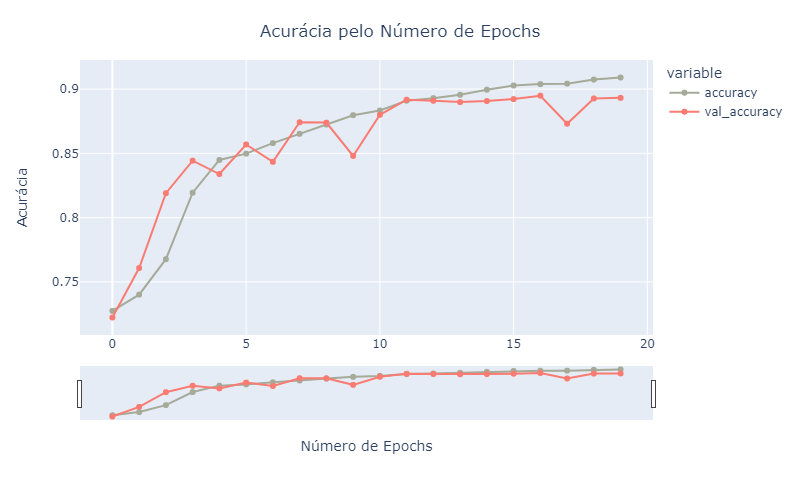
\includegraphics[scale=0.55]{./figs/lstm_acuracy.png}
    \caption{Relação acurácia por \textit{epochs}}
    \label{fig:lstmacuracy}
\end{figure}

A rede neural LSTM tem uma acurácia muito alta, mas um tempo de execução extremamente longo, o que pode torná-la impraticável para muitas aplicações em tempo real. No entanto, para aplicações onde a precisão é o fator mais importante, como diagnóstico médico ou detecção de fraudes financeiras, esse modelo pode ser a melhor opção.

Em redes neurais, uma época refere-se a um ciclo completo de treinamento de todos os dados de treinamento disponíveis na rede. Durante cada um desses ciclos, os dados são passados pela rede em lotes (ou \textit{batch}), a rede faz previsões para cada lote, compara as previsões com as respostas corretas e atualiza os pesos e bias da rede para minimizar o erro (ou função de custo) entre as previsões e as respostas corretas.

Após uma época completa, a rede é capaz de fazer previsões melhores do que antes do treinamento começar. À medida que o treinamento continua avançando, as previsões melhoram gradualmente até que a rede esteja suficientemente treinada para fazer previsões precisas sobre novos dados.

O número de \textit{epochs} que uma rede neural precisa para ser treinada depende do problema e da complexidade da rede. Um número muito baixo de \textit{epochs} pode resultar em previsões imprecisas, enquanto um número muito alto pode levar a um excesso de ajuste (overfitting) dos dados de treinamento.

Por fim, faz-se um comparativo entre a acurácia de todos os modelos para o \textit{dataset} de treino e tem-se a \autoref{tab:time} com o tempo de execução para cada um dos modelos.

\begin{figure}[H]
    \centering
    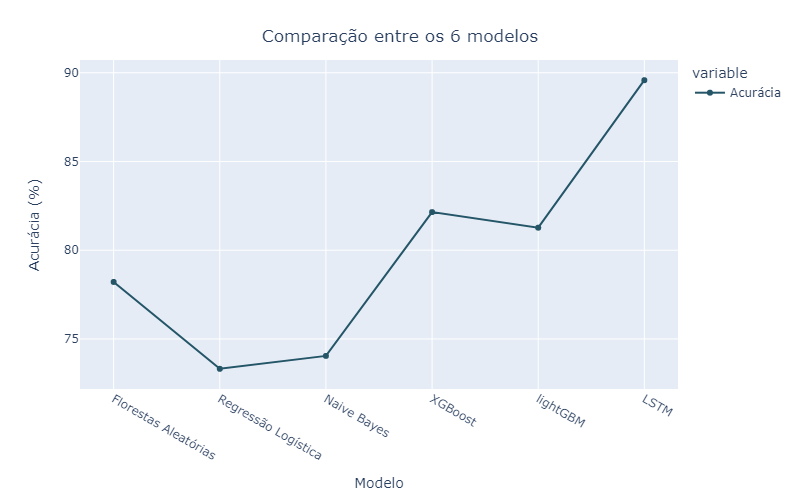
\includegraphics[scale=0.55]{./figs/comparative.png}
    \caption{Comparação de acurácia entre modelos}
    \label{fig:comparative}
\end{figure}

\begin{table}[H]
    \centering
    \small
    \begin{tabular}{c|cccccc}
        \hline
        { modelo}        & { Reg. Logística} & { F. Aleatórias} & { XGBoost} & { Naive Bayes} & LightGBM & LSTM \\ \hline \hline
        { Tempo (s)}     & { 21.5}           & { 1.5}           & { 3.0}     & { 0.1}         & {1.5}    & 1500 \\ \hline
        { Acurácia (\%)} & { 73.3}           & { 78.2}          & { 82.1}    & { 74.0}        & 81.3     & 90.0 \\
    \end{tabular}
    \caption{Tempo de execução/Acurácia dos modelos avaliados em teste}
    \label{tab:time}
\end{table}

Embora a acurácia seja uma métrica importante, ela pode não ser suficiente para avaliar completamente o desempenho de um modelo em alguns casos. Por exemplo, em problemas de classificação desbalanceados, onde uma classe é muito mais comum do que a outra, a acurácia pode ser enganosa. Nesses casos, outras métricas, como a precisão, a recall e a F1-score podem ser mais úteis.

Além disso, a acurácia não leva em consideração a gravidade dos erros de classificação. Por exemplo, em um problema de diagnóstico médico, um falso negativo pode ter consequências mais graves do que um falso positivo. Portanto, é importante avaliar o desempenho do modelo em relação a métricas que levam em consideração a gravidade dos erros de classificação, como a matriz de confusão.

Isso posto, avaliou-se os modelos também pela matriz de confusão e curva ROC.


\begin{figure}[H]
    \centering
    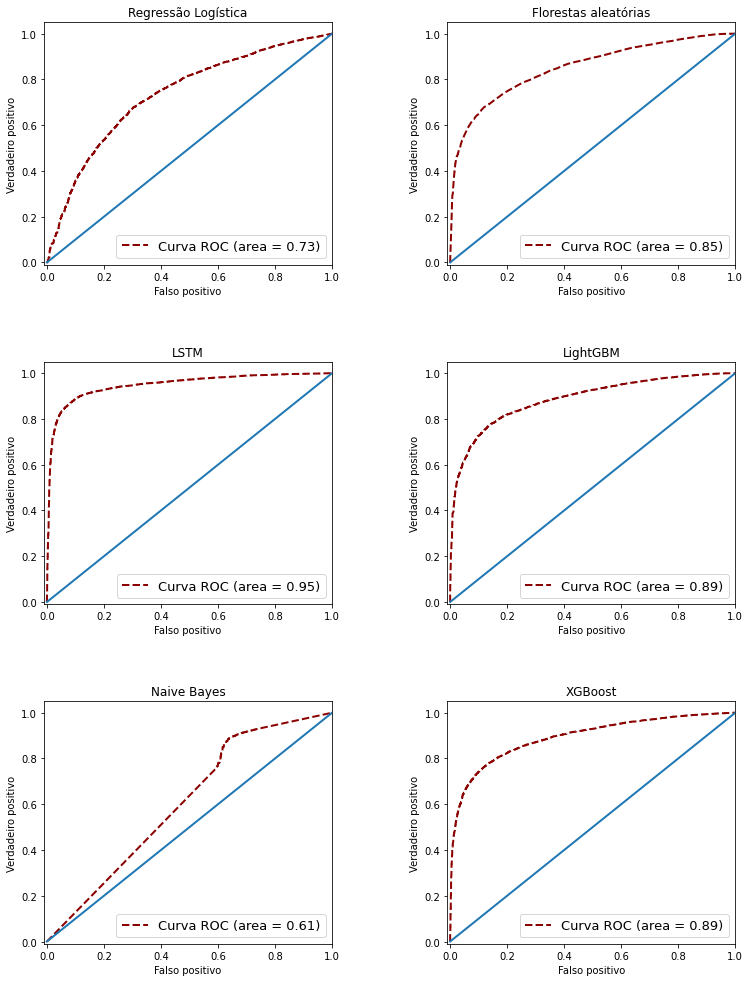
\includegraphics[scale=0.6]{./figs/roc_v.png}
    \caption{Curvas ROC dos modelos utilizados}
    \label{fig:roccurve}
\end{figure}

\begin{figure}[H]
    \centering
    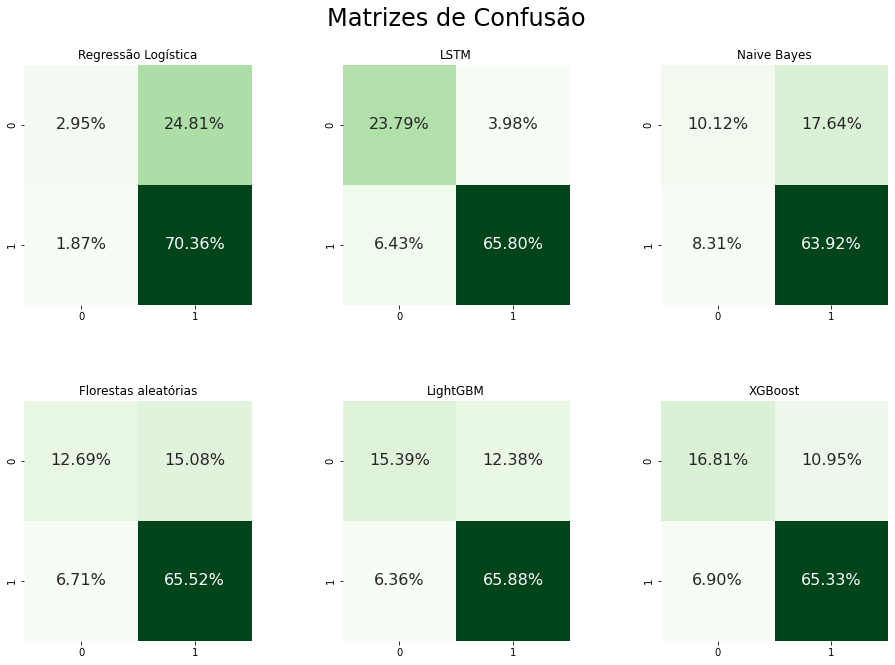
\includegraphics[scale=0.5]{./figs/confusion.png}
    \caption{Matrizes de confusão dos modelos utilizados}
    \label{fig:mconfusion}
\end{figure}

A matriz de confusão é uma tabela que mostra o número de exemplos que foram classificados corretamente e incorretamente pelo modelo, divididos em quatro categorias: verdadeiro positivo (TP-00), verdadeiro negativo (TN-11), falso positivo (FP-10) e falso negativo (FN-01). A partir dessa matriz, várias métricas de desempenho podem ser calculadas, incluindo a acurácia, precisão e recall. A matriz de confusão pode ajudar a identificar padrões de erros comuns que o modelo está cometendo.

Essas três equações podem ser representadas da seguinte forma:

\begin{equation}
    \text{Acurácia} = \frac{\text{VP} + \text{VN}}{\text{VP} + \text{FP} + \text{VN} + \text{FN}}
\end{equation}

\begin{equation}
    \text{Precisão} = \frac{\text{VP}}{\text{VP} + \text{FP}}
\end{equation}

\begin{equation}
    \text{Recall} = \frac{\text{VP}}{\text{VP} + \text{FN}}
\end{equation}

Já a curva ROC (\textit{Receiver Operating Characteristic}) é uma curva que mostra a relação entre a taxa de verdadeiros positivos (TPR) e a taxa de falsos positivos (FPR) para diferentes valores de limiar de classificação. Em outras palavras, a curva ROC mostra como o modelo se comporta em termos de sensibilidade e especificidade para diferentes pontos de corte de probabilidade de classificação. Quanto mais próxima a curva ROC estiver do canto superior esquerdo, melhor será o desempenho do modelo. A área sob a curva ROC (AUC-ROC) é uma medida resumida da performance do modelo, sendo que o valor máximo é 1,0, o que indica uma performance perfeita.

Ao avaliar a curva ROC, podemos observar que a LSTM também apresentou a maior área sob a curva, indicando uma maior capacidade de distinguir entre as classes. Esse resultado é consistente com a análise das matrizes de confusão, que mostraram que a LSTM teve o melhor desempenho na classificação correta das amostras.

O XGBoost e LightGBM também apresentaram resultados promissores, tendo o XGBoost uma acurácia um pouco melhor de $82\%$ e uma área sob a curva ROC de 0,89. No entanto, as matrizes de confusão indicaram que os modelos cometeram mais erros do que a LSTM na classificação de algumas amostras.

Por outro lado, a regressão logística e o Naive Bayes apresentaram as piores performances, com acurácias de $73\%$ e $74\%$, respectivamente, e áreas sob a curva ROC menores do que os outros modelos avaliados.

A escolha entre usar a matriz de confusão e/ou a curva ROC depende do objetivo do problema e da preferência do usuário. Enquanto a matriz de confusão oferece informações detalhadas sobre o desempenho do modelo em cada classe, a curva ROC pode ser mais útil para escolher o melhor modelo entre vários modelos ou ajustar o ponto de corte de classificação para atingir um determinado objetivo, como minimizar a taxa de falsos positivos ou maximizar a taxa de verdadeiros positivos.



% ---------------------------------------------------------------------------- %
\section{Conclusões}
\label{sec:conclu}

Com base na análise dos resultados, podemos concluir que a rede neural artificial LSTM apresentou a melhor performance em relação aos outros algoritmos de \textit{machine learning} avaliados. A acurácia da LSTM foi de $90\%$, o que indica que o modelo foi capaz de classificar corretamente a grande maioria dos dados.

Ao avaliar a curva ROC, podemos observar que a LSTM também apresentou a maior área sob a curva, indicando uma maior capacidade de distinguir entre as classes. Esse resultado é consistente com a análise das matrizes de confusão, que mostraram que a LSTM teve o melhor desempenho na classificação correta das amostras.

O XGBoost também apresentou resultados promissores, com uma acurácia de $82\%$ e uma área sob a curva ROC de 0,89. No entanto, as matrizes de confusão indicaram que o modelo cometeu mais erros do que a LSTM na classificação de algumas amostras.

Por outro lado, a regressão logística e o Naive Bayes apresentaram as piores performances, com acurácias de $73\%$ e $61\%$, respectivamente, e áreas sob a curva ROC menores do que os outros modelos avaliados.

Se tratando de \textit{tradeoff}, na prática, muitas vezes é necessário encontrar um equilíbrio entre a rapidez da resposta e a precisão do modelo. Isso ocorre porque muitas aplicações em tempo real exigem que a resposta seja obtida em um curto espaço de tempo, enquanto outras aplicações, como pesquisa médica ou financeira, priorizam a precisão.

A escolha do modelo ideal depende de vários fatores, como o tamanho dos dados, a complexidade do problema e a disponibilidade de recursos de computação. Modelos mais complexos, como as redes neurais, podem ter uma acurácia muito alta, mas exigem uma grande quantidade de tempo de processamento, enquanto modelos mais simples, como regressão logística ou Naive Bayes, têm tempos de processamento menores, mas podem ter uma acurácia menor.

As Florestas Aleatórias e o XGBoost são modelos intermediários em termos de complexidade e tempo de execução. Esses modelos podem ser mais adequados para muitas aplicações, pois têm uma acurácia razoável e um tempo de execução curto o suficiente para muitas tarefas em tempo real.

No caso específico apresentado no trabalho, a regressão logística tem um tempo de execução muito maior do que os outros modelos, o que pode ser um fator limitante em muitas aplicações. Por outro lado, o Naive Bayes tem um tempo de execução muito curto, mas também tem a menor acurácia entre os modelos apresentados.

A rede neural LSTM tem uma acurácia muito alta, mas um tempo de execução extremamente longo, o que pode torná-la impraticável para muitas aplicações em tempo real. No entanto, para aplicações onde a precisão é o fator mais importante, como diagnóstico médico ou detecção de fraudes financeiras, esse modelo pode ser a melhor opção.

Outrossim, é necessário destacar que o XGBoost possui algumas vantagens em relação a redes neurais como a LSTM.

Uma das delas é a sua capacidade de lidar com dados heterogêneos e faltantes de forma eficiente, o que pode ser um desafio para redes neurais. Além disso, com a visão de um negócio, onde a velocidade é importante, o XGBoost é um modelo mais simples e rápido de treinar do que redes neurais, o que pode ser uma vantagem em cenários em que o tempo e recursos computacionais são limitados.

O XGBoost também apresenta interpretabilidade, uma vez que ele permite identificar as variáveis mais importantes para a classificação dos dados. As redes neurais, embora apresentem alta performance em muitas tarefas, são frequentemente consideradas caixas pretas, dificultando a interpretação dos resultados.

Portanto, embora a LSTM tenha apresentado a melhor performance na análise classificatória realizada, o XGBoost pode ser uma boa opção em cenários em que a interpretabilidade e o processamento de dados faltantes são prioridades.

Por outro lado, a LSTM consegue lidar com dados sequenciais e com dependências de longo prazo, o que pode ser um desafio para algoritmos de aprendizado de máquina tradicionais. Isso torna a LSTM uma escolha popular para tarefas de processamento de linguagem natural, reconhecimento de fala, análise de séries temporais, entre outras aplicações em que o histórico de dados é importante. Além disso, ela é capaz de aprender padrões complexos em dados sequenciais sem a necessidade de engenharia manual de características, o que pode ser um processo demorado e sujeito a erros nos outros algoritmos, incluindo o XGBoost. Isso pode resultar em um desempenho melhor para a LSTM em tarefas em que há uma grande quantidade de dados sequenciais.

Outra vantagem da LSTM é a sua capacidade de lidar com dados de entrada de diferentes tipos e tamanhos, como sequências de palavras, imagens e dados numéricos. Isso torna a LSTM uma escolha popular em aplicações em que os dados podem ter diferentes formatos, como reconhecimento de fala e tradução automática.

Para análise de sentimentos em reviews de usuários, a LSTM pode ser mais vantajosa do que o XGBoost. Isso ocorre porque as análises de sentimentos geralmente envolvem dados sequenciais, como sequências de palavras ou frases em uma revisão, e as LSTMs são projetadas especificamente para trabalhar com dados sequenciais e são capazes de aprender padrões em sequências de dados de maneira mais eficiente do que algoritmos de aprendizado de máquina.

Além disso, as LSTMs têm a capacidade de capturar dependências de longo prazo nos dados sequenciais, o que pode ser importante para a análise de sentimentos em reviews de usuários, já que as opiniões dos usuários muitas vezes são expressas em frases e parágrafos complexos e detalhados.

No entanto, é importante ressaltar que a escolha do algoritmo de \textit{machine learning} depende do conjunto de dados e do problema em questão. Algoritmos mais simples podem ser mais eficazes em alguns cenários, enquanto algoritmos mais complexos, como redes neurais, podem ser necessários para lidar com dados mais complexos e variáveis. Em última análise, a escolha do algoritmo deve ser baseada em uma análise cuidadosa dos dados e das necessidades específicas do problema em questão.
% ---------------------------------------------------------------------------- %

% ---------------------------------------------------------------------------- %
% Bibliografia
\bibliographystyle{natbib} % citação bibliográfica textual plainnat-ime,natbib
\bibliography{ref}  % associado ao arquivo: 'bibliografia.bib'
\nocite{*}

\end{document}